\begin{figure*}[t]
\centering
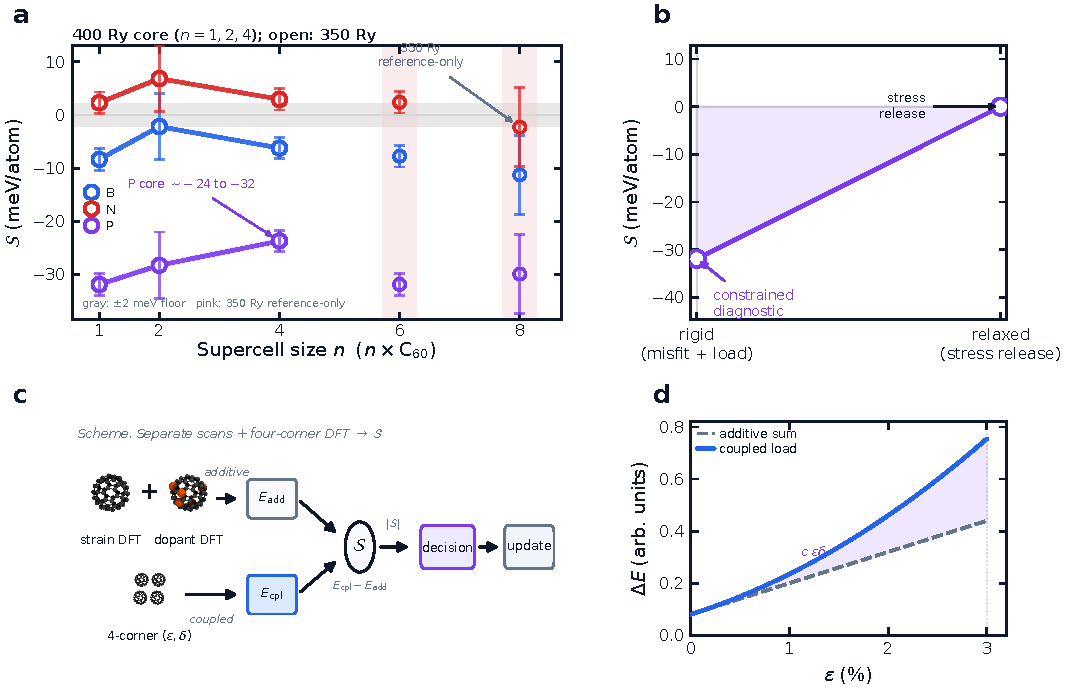
\includegraphics[width=\textwidth]{figures/out/figure_prb_2_synergy.pdf}
\caption{\label{fig:synergy}Additive strain--dopant screening fails under constrained load.
(a)~Fifteen periodic $+3$\% $\mathcal{S}(n,\delta)$ values vs.\ supercell size (markers: DFT; error bars and gray band: $\pm 2$~meV/atom protocol floor; Tables~\ref{tab:sigma_S} and~\ref{tab:sgrid}). $|\mathcal{S}|$ does not fall as $1/n$: P remains ${\sim}-24$ to $-32$~meV/atom through $n{=}8$; B stays negative at $-2$ to $-11$; N changes sign at $n{=}8$. Only P lies far outside the band at every size; N is at its edge, so the audit resolves a stratification and not a uniform failure of additivity. No $\mathcal{S}_\infty$ extrapolation.
(b)~Protocol bound, not a second size-scaling panel: periodic $n{=}1$ P at $+3$\%, rigid vs.\ ionically relaxed $\mathcal{S}$ (near zero after stress release). The tetramer sign reversal in Table~\ref{tab:relax} is a different system.
(c)~Definition: additive sum of strain-only and substitution-only increments vs.\ the coupled four-corner total; $\mathcal{S}$ is that gap [Eq.~\eqref{eq:four_corner}].
(d)~Schematic $E(\epsilon)$ at fixed composition: the bilinear $c\,\epsilon\delta$ term bends the coupled path away from the additive sum (cartoon, not a DFT fit).}
\end{figure*}
